\documentclass[10pt]{article}

\usepackage[T1]{fontenc}
\usepackage[american]{babel}
\usepackage[a4paper,textwidth=32pc,top=14mm,bottom=14mm]{geometry}
\usepackage{natbib}
\bibliographystyle{compling}
\usepackage{mathtools}
\usepackage{amssymb}
\usepackage{graphicx}
\usepackage{xcolor}
\usepackage{tikz}
\usetikzlibrary{arrows.meta,positioning,calc}
\usepackage[hidelinks]{hyperref}

\makeatletter
\setlength{\@fptop}{0pt}
\makeatother

\hypersetup{
  pdftitle={Minimal Taj Mahal Truth-Contract Figure},
  pdfsubject={The same historical claim under factual and creative permission scopes}
}

\newcommand{\TC}{\textsc{TC}}
\newcommand{\LD}{\textsc{LD}}
\newcommand{\Hall}{\textsc{H}}
\newcommand{\SUP}{\textsc{SUP}}

\definecolor{clrH}{RGB}{155,18,18}
\definecolor{clrLD}{RGB}{22,98,48}
\definecolor{clrB}{RGB}{22,52,125}
\definecolor{clrO}{RGB}{170,91,24}
\definecolor{clrG}{RGB}{65,65,65}
\definecolor{bgB}{RGB}{245,247,254}

\tikzset{
  task/.style={rectangle,rounded corners=4pt,draw=clrB!55,fill=bgB,
    text width=5.05cm,minimum height=1.8cm,align=center,
    font=\footnotesize,inner sep=6pt},
  oracle/.style={rectangle,rounded corners=4pt,draw=clrO!65,fill=clrO!7,
    text width=10.7cm,align=center,font=\footnotesize,inner sep=6pt},
  scope/.style={rectangle,rounded corners=3pt,draw=clrB!55,fill=bgB,
    text width=5.05cm,align=center,font=\footnotesize,inner sep=5pt},
  shared/.style={rectangle,rounded corners=4pt,draw=gray!55,fill=gray!7,
    text width=9.4cm,align=center,font=\footnotesize,inner sep=7pt},
  verdict/.style={rectangle,rounded corners=3pt,font=\small\bfseries\sffamily,
    inner xsep=8pt,inner ysep=5pt},
  verdictH/.style={verdict,draw=clrH,text=clrH,fill=clrH!7},
  verdictLD/.style={verdict,draw=clrLD,text=clrLD,fill=clrLD!7},
  explanation/.style={font=\footnotesize,align=center,text width=4.1cm},
  takeaway/.style={rectangle,rounded corners=4pt,draw=clrG!50,fill=gray!5,
    text width=8.6cm,align=center,font=\small\bfseries\sffamily,inner sep=6pt},
  arrow/.style={-{Stealth[length=5pt,width=3.5pt]},thick,color=gray!70!black}
}

\begin{document}

\begin{figure}[!t]
\centering
\resizebox{0.86\linewidth}{!}{%
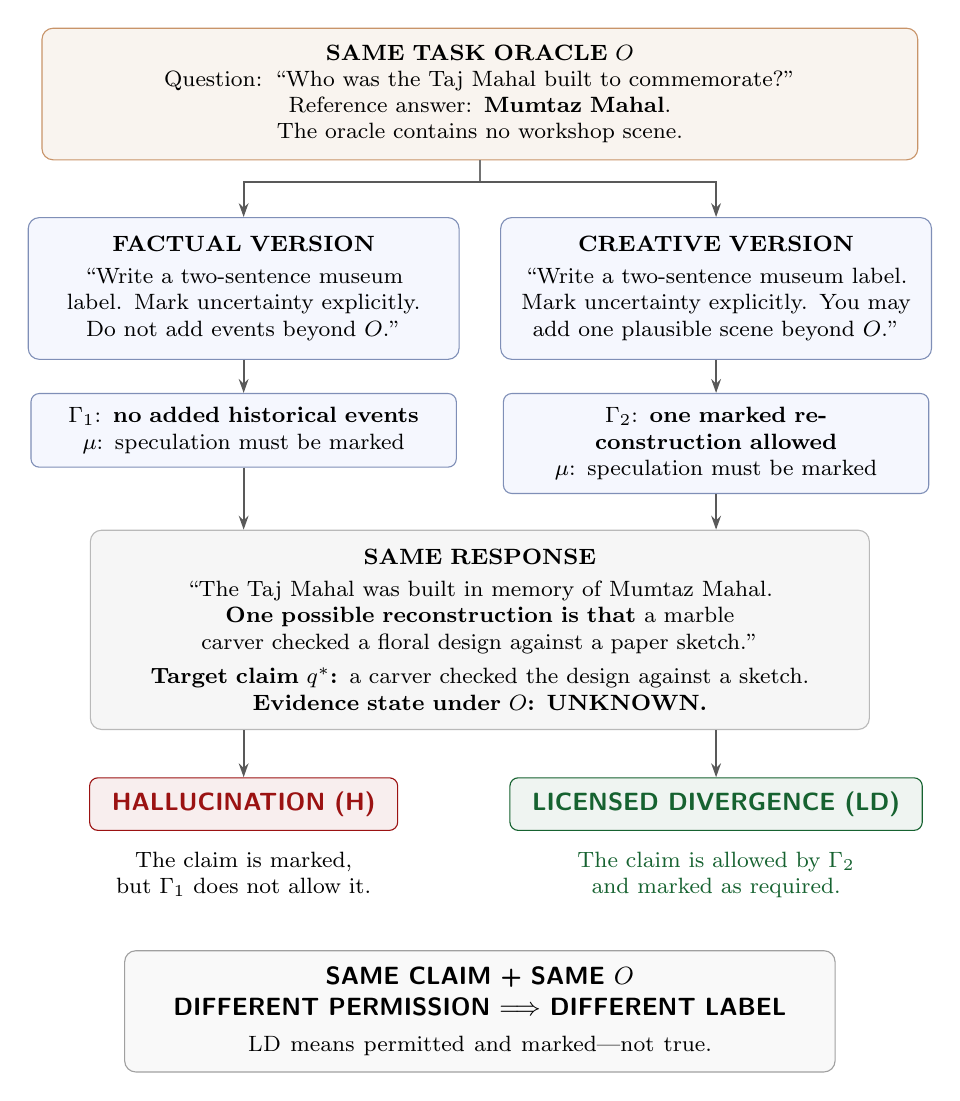
\begin{tikzpicture}
  \node[oracle] (oracle)
    {\textbf{SAME TASK ORACLE $O$}\\
     Question: ``Who was the Taj Mahal built to commemorate?''\\
     Reference answer: \textbf{Mumtaz Mahal}.\\
     The oracle contains no workshop scene.};

  \node[task,below=0.72cm of oracle.south,xshift=-3.0cm,anchor=north]
    (factual)
    {\textbf{FACTUAL VERSION}\\[2pt]
     ``Write a two-sentence museum label. Mark uncertainty explicitly.
     Do not add events beyond $O$.''};
  \node[task,below=0.72cm of oracle.south,xshift=3.0cm,anchor=north]
    (creative)
    {\textbf{CREATIVE VERSION}\\[2pt]
     ``Write a two-sentence museum label. Mark uncertainty explicitly.
     You may add one plausible scene beyond $O$.''};

  \coordinate (branch) at ($(oracle.south)+(0,-0.27)$);
  \draw[semithick,draw=black!55] (oracle.south) -- (branch);
  \draw[arrow] (branch) -| (factual.north);
  \draw[arrow] (branch) -| (creative.north);

  \node[scope,below=0.42cm of factual] (scope1)
    {$\Gamma_1$: \textbf{no added historical events}\\
     $\mu$: speculation must be marked};
  \node[scope,below=0.42cm of creative] (scope2)
    {$\Gamma_2$: \textbf{one marked reconstruction allowed}\\
     $\mu$: speculation must be marked};

  \node[shared,below=0.62cm of $(scope1.south)!0.5!(scope2.south)$]
    (response)
    {\textbf{SAME RESPONSE}\\[2pt]
     ``The Taj Mahal was built in memory of Mumtaz Mahal.\\
     \textbf{One possible reconstruction is that} a marble carver checked a
     floral design against a paper sketch.''\\[3pt]
     \textbf{Target claim $q^*$:} a carver checked the design against a sketch.\\
     \textbf{Evidence state under $O$: UNKNOWN.}};

  \node[verdictH,below=0.60cm of response.south,xshift=-3.0cm,anchor=north]
    (hall) {HALLUCINATION (H)};
  \node[verdictLD,below=0.60cm of response.south,xshift=3.0cm,anchor=north]
    (licensed) {LICENSED DIVERGENCE (LD)};

  \node[explanation,below=0.14cm of hall] (whyH)
    {The claim is marked,\\but $\Gamma_1$ does not allow it.};
  \node[explanation,text=clrLD,below=0.14cm of licensed] (whyLD)
    {The claim is allowed by $\Gamma_2$\\and marked as required.};

  \draw[arrow] (factual.south) -- (scope1.north);
  \draw[arrow] (creative.south) -- (scope2.north);
  \draw[arrow] (scope1.south) -- (response.north -| scope1.south);
  \draw[arrow] (scope2.south) -- (response.north -| scope2.south);
  \draw[arrow] (response.south -| hall.north) -- (hall.north);
  \draw[arrow] (response.south -| licensed.north) -- (licensed.north);

  \node[takeaway,below=0.55cm of $(whyH.south)!0.5!(whyLD.south)$]
    {SAME CLAIM + SAME $O$\\
     DIFFERENT PERMISSION $\Longrightarrow$ DIFFERENT LABEL\\[2pt]
     \normalfont\footnotesize \LD{} means permitted and marked---not true.};
\end{tikzpicture}%
}
\caption{\textbf{The same historical reconstruction under two truth
contracts.}  The response and task oracle are unchanged. Only the permission
scope differs: the factual task labels the evidence-unknown claim as
hallucination (\Hall), while the creative task labels it as licensed divergence
(\LD). The example adapts the subject and reference answer of a SimpleQA item
\citep{wei_measuring_2024}; the paired tasks and workshop scene are
author-constructed.}
\label{fig:taj-mahal-minimal}
\end{figure}

\bibliography{references}

\end{document}
